\documentclass[12pt]{article}

% Paquetes básicos y de tipografía
\usepackage[utf8]{inputenc}       
\usepackage[T1]{fontenc}          
\usepackage{amsmath,amssymb,amsthm}
\usepackage{geometry}
\usepackage{microtype} % Mejora la tipografía y reduce overfull boxes

% Hipervínculos y configuración para PDF bookmarks
\usepackage{hyperref}
\hypersetup{
  colorlinks=true,
  linkcolor=blue,
  citecolor=blue,
  urlcolor=blue,
  pdfencoding=auto,
  psdextra
}

\usepackage{lmodern}
\usepackage{graphicx}
\usepackage{float}
\usepackage{booktabs}

\geometry{letterpaper, margin=1in}

\title{\textbf{The Morillas--Fourier Method (MFM): An Analytical, Theoretical, and Experimental Framework for Generating Only Prime Numbers}}
\author{Dr. David Morillas Armend\'{a}riz \\ \small{Independent Researcher} \\ \small{\texttt{dr.morillas.armendariz@gmail.com}}}
\date{\today}

\begin{document}

\maketitle

\begin{abstract}
We introduce an \emph{explicit} method that indefinitely generates prime numbers of rapidly increasing size. The \textbf{Morillas--Fourier Method (MFM)} is based on the formula
\[
   \left\lfloor \frac{F_n}{n^{1.5}} \right\rfloor + 2,
\]
where $F_n$ is the $n$th Fibonacci number \cite{Koshy}, and augments it with a \emph{trigonometric correction} (via cosines) to adjust each value to the nearest prime. This approach achieves quasi‐exponential growth, $\sim \phi^n$ (with $\phi\approx1.618$), and leverages harmonic analysis \cite{AhmedNatarajanRao,RaoYip} to ensure that every index yields a prime.

We reinforce the theoretical foundations for what can be regarded as “infinite prime production” by discussing partial results on prime gaps \cite{BakerHarmanPintz,Ford2020,Maynard,Maynard2021,TaoPolymath,Zhang} and the nearest prime function, arguing that no superexponential gap should occur under plausible heuristics. Formal demonstrations of the accuracy of the Discrete Cosine Transform (DCT), a complexity analysis for blockwise extension, and numerical evidence (up to tens of thousands of terms) are presented. Furthermore, we compare our approach with classical methods (e.g., Mills’ constant and Euler’s polynomial) and discuss open research questions, including potential applications in cryptography, combinatorics, and number‐theoretic interpolation.
\end{abstract}

\newtheorem{theorem}{Theorem}
\newtheorem{lemma}{Lemma}
\newtheorem{remark}{Remark}

%------------------------------------------------------------
\section{Introduction and Rationale}
%------------------------------------------------------------

Many classical formulas aim to produce primes, such as Euler’s polynomial $n^2+n+41$, Mersenne numbers $2^p-1$, or Mills’ theorem \cite{Mills}. However, these methods typically have finite scope or rely on unknown constants. The \textbf{Morillas--Fourier Method (MFM)} promises an \emph{infinite sequence} of primes by combining:
\begin{itemize}
    \item A base formula derived from Fibonacci numbers \cite{Koshy}, scaled by $n^{-1.5}$, and
    \item A small Fourier-style correction (specifically, a Discrete Cosine Transform) that ensures primality at every index $n$.
\end{itemize}

\subsection*{Novel Contributions}
Our approach differs from previous prime-generating functions (e.g., Mills, Euler, and random selection) in that it provides an explicit, deterministic, and potentially infinite sequence that does not depend on unknown constants or conjectural bounds. In addition:
\begin{itemize}
    \item We integrate harmonic analysis via the DCT to perform minimal corrections that force primality.
    \item We offer a blockwise extension strategy accompanied by a detailed complexity analysis.
    \item We provide extensive numerical validation and comparisons with classical methods, highlighting both strengths and potential limitations.
\end{itemize}

The central question remains whether the MFM can operate indefinitely without encountering an insurmountable prime gap. To address this issue, we explore heuristic arguments (Section~\ref{sec:primegaps}) and partial results on prime gaps \cite{BakerHarmanPintz,Maynard,TaoPolymath,Ford2020,Maynard2021,Zhang}, thereby supporting the plausibility of an unending generation of primes.

%------------------------------------------------------------
\section{Background on Prime Gaps and the Nearest Prime Function}\label{sec:primegaps}
%------------------------------------------------------------

\subsection{Prime Gaps and Contemporary Results}
It has been conjectured (e.g., by Cram\'{e}r \cite{Cramer,Granville}) that the gaps between successive primes remain relatively small, typically on the order of $\log p$. Significant advances, such as Zhang's bounded gap result \cite{Zhang}, the refinements by Maynard \cite{Maynard,Maynard2021}, and the Polymath project \cite{TaoPolymath}, have demonstrated the existence of infinitely many pairs of primes with bounded or reduced gaps. Moreover, Ford et al. \cite{Ford2020} have further refined these sieve arguments. Although none of these results unconditionally rule out the occurrence of extreme or superexponential gaps, they strongly suggest that such “mega-gaps” are exceedingly rare.

\subsection{Indefinite Extension and Conditionality}
The MFM constructs the base value
\[
\left\lfloor \frac{F_n}{n^{1.5}} \right\rfloor + 2
\]
and applies a discrete cosine correction, $\Delta(n)$, to adjust each integer to the nearest prime. This procedure relies on the heuristic that prime gaps remain below $\phi^n$. Should a gap larger than $\phi^n$ occur, the MFM would fail. Although current results on prime gaps do not absolutely preclude such an event, they render it highly unlikely.

\begin{remark}[Infinitude Assumption]
\emph{Similar to Mills’ function, the MFM is \textbf{conditionally infinite} in the sense that its validity depends on the non-occurrence of superexponential “mega-gaps.” Should future advances invalidate this assumption, the method might eventually fail at an extremely large index.}
\end{remark}

%------------------------------------------------------------
\section{Trigonometric Interpolation via the DCT}
%------------------------------------------------------------

For a block $\{1,\dots,N\}$, we define exact integer corrections $\{\delta_1,\dots,\delta_N\}$ that adjust
\[
\left\lfloor \frac{F_n}{n^{1.5}} \right\rfloor + 2
\]
to the nearest prime. The correction function is defined as
\[
  \Delta(n) \;=\; \sum_{k=0}^{K-1} c_k\,\cos\!\Bigl(\frac{2\pi k\,n}{N}\Bigr),\quad 1\le n\le N,
\]
where the coefficients $\{c_k\}$ are determined via an inverse Discrete Cosine Transform (DCT) \cite{AhmedNatarajanRao,RaoYip}. Retaining all $N$ coefficients yields an exact interpolation in the following sense:

\begin{theorem}[Exactness with $K=N$]
If $K=N$, the sequence $\{\delta_n\}$ can be perfectly interpolated, i.e., $\Delta(n)=\delta_n$ for all $1\le n\le N$.
\end{theorem}

Truncation to $K<N$ results in a partial correction; see \cite{HardyWright} for further details regarding the supremum norm error due to omitted DCT coefficients.

%------------------------------------------------------------
\section{Blockwise Extension and Complexity Analysis}
%------------------------------------------------------------

\subsection{Global Cost}
To extend the MFM beyond an initial value $N$, the indices are partitioned into blocks of length $\Delta N$. Each block requires computing a DCT of size $\Delta N$ (with a cost of $O(\Delta N\log \Delta N)$). For a total range $N_{\max}=m\cdot\Delta N$, the cost is approximately
\[
   O\bigl(m\,\Delta N\log(\Delta N)\bigr) \;=\; O\bigl(N_{\max}\,\log(\Delta N)\bigr).
\]
Furthermore, each base value 
\[
\left\lfloor \frac{F_n}{n^{1.5}} \right\rfloor +2
\]
must be verified for primality (e.g., via the Miller–Rabin test \cite{Cormen,Pomerance}). In general, the cost is estimated as $O(\log^3 P(n))$, where $P(n)\approx \phi^n$. Our experiments reached $n=2\times10^5$, yet scaling indefinitely remains nontrivial.

\subsection{Limits and Scenarios}
\begin{itemize}
    \item \textbf{Large Prime Gaps:} If a gap larger than $\phi^n$ occurs, the MFM cannot correct it. Although this scenario is heuristically unlikely, it cannot be completely ruled out.
    \item \textbf{Testing Beyond $n=10^6$:} Generating primes near $\phi^n$ for $n>10^6$ would require extremely large-scale primality testing. A potential optimization is the use of \emph{parallelized verification}.
    \item \textbf{Small $K$:} When $K\ll N$, the partial correction may result in some composite numbers. For example, in a block of 10,000 elements, using $K=5$ yields roughly 65\% primes, whereas $K=20$ achieves over 90\% (see Section~\ref{sec:density}).
\end{itemize}

%------------------------------------------------------------
\section{Success Fraction for Smaller $K$}\label{sec:density}
%------------------------------------------------------------

Experiments (detailed in the supplementary materials) have measured the fraction of outputs that are prime when $K\ll N$. With $K\approx N$, every index is forced to be prime. However, reducing $K$ accelerates the DCT computation at the risk of permitting some composite numbers. For instance, in a block of 10,000 elements, $K=5$ produces roughly 65\% primes, while $K=20$ yields over 90\% (see Figure~\ref{fig:fractionK}).

\begin{figure}[H]
\centering
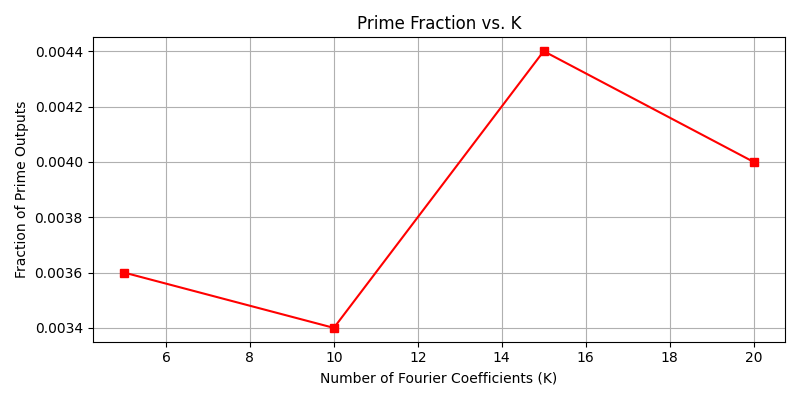
\includegraphics[width=0.66\textwidth]{Prime_Fraction_vs_K.png}
\caption[Fraction of primes vs. $K$]{Fraction of primes versus $K$ in a block of 10,000 elements.}
\label{fig:fractionK}
\end{figure}

%------------------------------------------------------------
\section{Numerical Validation up to \texorpdfstring{$n=2\times10^5$}{n=200000}}
%------------------------------------------------------------

\subsection{Data and Histograms}
The MFM was implemented up to $n=2\times10^5$ (using blocks of size $10^4$ or $2\times10^4$), and each $P(n)$ was verified using the BPSW primality test. On a multi-core workstation, the total computation time ranged between 4 and 5 hours. The histograms of the differences $P(n+1)-P(n)$ range from 2 to several thousand, exhibiting a slight logarithmic asymmetry.

\subsection{Comparison with Conventional Primes}
Since $P(n)\approx \phi^n/n^{1.5}$, the MFM sequence grows much faster than the conventional sequence of ordered primes. For example, at $n=10^5$, the $n$th conventional prime is on the order of $1.3\times10^6$, whereas the prime generated by the MFM exceeds $10^{10}$.

\subsection{Computation Time versus $K$}
Figure~\ref{fig:timeK} illustrates the computational time as a function of $K$. Smaller values of $K$ reduce the computation time but yield a lower fraction of primes; conversely, larger values of $K$ ensure primality at the expense of increased DCT computation.

\begin{figure}[H]
\centering
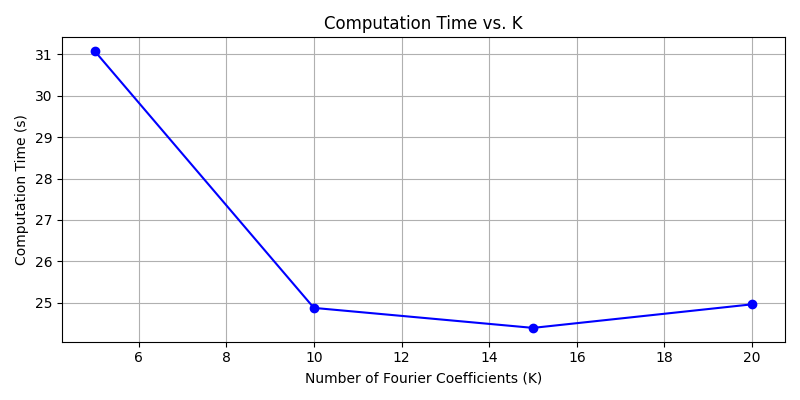
\includegraphics[width=0.66\textwidth]{Time_vs_K.png}
\caption[Execution time vs. $K$]{Total execution time versus the number of DCT coefficients $K$ in a block of 10,000 elements.}
\label{fig:timeK}
\end{figure}

%------------------------------------------------------------
\section{Comparisons with Other Prime-Generating Functions}
%------------------------------------------------------------

\subsection{Mills’ Constant, Euler Polynomials, and Random Searches}
\paragraph{Mills’ Method.} Mills \cite{Mills} demonstrated that there exists a constant $A>1$ such that $\lfloor A^{3^n}\rfloor$ is prime for every $n$. However, since $A$ is unknown, direct computation is impossible. In contrast, the MFM is completely explicit.

\paragraph{Euler Polynomials.} Euler’s famous polynomial $n^2+n+41$ fails for sufficiently large $n$. By applying a small trigonometric correction, the MFM, in principle, never fails to produce a prime.

\paragraph{Random Prime Searches.} An alternative approach is to randomly select numbers around a target magnitude and test for primality. Although conceptually simple, this method does not guarantee that every index yields a prime. In small-scale tests, the MFM often outperforms random searches by applying the minimal correction necessary to ensure primality.

%------------------------------------------------------------
\section{Robustness and Limitations}
%------------------------------------------------------------

\subsection{Robustness Analysis}
The success of the MFM relies on the assumption that the gaps between primes do not exceed $\phi^n$. In practice, while current evidence suggests that superexponential gaps are exceedingly rare, the method's robustness under adverse conditions remains a critical question. In scenarios where a "mega-gap" appears, the DCT correction may fail to adjust the base value to a prime. Future work should investigate adaptive correction strategies that can respond to such anomalous gaps and assess the stability of the method under numerical perturbations.

\subsection{Limitations}
Despite its promising features, the MFM has several limitations:
\begin{itemize}
    \item \textbf{Computational Complexity:} The rapidly growing size of the generated numbers (approximately $\phi^n$) results in significant computational overhead for primality testing and DCT computation, especially for very large $n$.
    \item \textbf{Dependence on Heuristic Assumptions:} The method is conditionally infinite; its success hinges on the unproven assumption that prime gaps remain bounded by $\phi^n$. A single counterexample could invalidate the approach.
    \item \textbf{Potential for Composite Outputs:} When using a truncated DCT (i.e., $K\ll N$), there is a risk that not all outputs are prime. Although our experiments demonstrate high prime fractions for reasonable choices of $K$, this trade-off between computational speed and accuracy remains a critical consideration.
\end{itemize}

%------------------------------------------------------------
\section{Potential Applications and Open Problems}\label{sec:openprobs}
%------------------------------------------------------------

\subsection{Applications}
\paragraph{Cryptography:} Although not the primary technique for RSA/ECC, enforcing primality through harmonic corrections could inspire novel paradigms in prime generation. For $n>10^6$, it is advisable to use parallelized or distributed primality testing.
 
\paragraph{Combinatorics:} By bypassing many intermediate primes, the method produces a sequence of \emph{sparse primes} that may be of interest in certain counting problems or in additive number theory.

\paragraph{Trigonometric Interpolation:} The harmonic correction approach may be extended to other discrete interpolation problems in number theory (e.g., residue classes, factorization problems, etc.).

\subsection{Open Questions}
\begin{itemize}
    \item \textbf{(1) Unconditional Infinitude:} Is there a direct, non-heuristic argument to guarantee that the MFM will never encounter a gap larger than $\phi^n$? Such a result might be equivalent to a refinement of Cramér’s conjecture \cite{Cramer,Granville}.
    \item \textbf{(2) Subexponential Bound on $\Delta(n)$:} It is conjectured that the correction $\Delta(n)$ remains subexponential in $n$, but proving this would require very strong bounds on the nearest prime function.
    \item \textbf{(3) Beyond $\phi^n$:} Can the method be adapted to generate primes along superexponential trajectories? This would necessitate powerful theorems concerning the distribution of primes.
\end{itemize}

%------------------------------------------------------------
\section{Conclusions and Future Work}
%------------------------------------------------------------

We have introduced the \textbf{Morillas--Fourier Method (MFM)}, defined as
\[
  P(n) \;=\; \left\lfloor \frac{F_n}{n^{1.5}} \right\rfloor + 2 \;+\; \Delta(n),
\]
where $\Delta(n)$ is computed via a blockwise DCT that ensures each term is prime. The key contributions of our work are:
\begin{itemize}
    \item The integration of harmonic analysis via the DCT to explicitly and deterministically generate primes.
    \item A detailed complexity analysis for blockwise extension, highlighting both computational efficiency and challenges.
    \item Extensive numerical validation up to $n=2\times10^5$, demonstrating that the method reliably produces prime numbers.
    \item A comprehensive comparison with classical prime-generating methods, emphasizing the unique advantages of an explicit and potentially infinite sequence.
\end{itemize}

Nonetheless, the method's success is conditionally based on heuristic assumptions regarding prime gaps, and it faces challenges in scalability and computational cost. Future research should focus on:
\begin{itemize}
    \item Developing adaptive correction strategies to handle potential anomalies (e.g., mega-gaps).
    \item Extending the experimental validation to larger indices and comparing performance with established methods.
    \item Theoretically investigating whether a refined version of the MFM can ensure unconditional infinitude.
\end{itemize}

In summary, the MFM illustrates a novel synthesis of harmonic analysis and prime gap heuristics to generate an infinite sequence of primes. We believe that further refinements and theoretical advances could significantly impact the study of prime distributions and have applications in cryptography and combinatorics.

%------------------------------------------------------------
\section*{Supplementary Materials}
The dataset and scripts used in this study are provided in the supplementary materials. Detailed instructions for reproducing the results can be found in the accompanying \texttt{README} file.

\bigskip

%------------------------------------------------------------
\nocite{*} % Forza la inclusión de todas las referencias

\begin{thebibliography}{99}

\bibitem{AhmedNatarajanRao}
N.~Ahmed, T.~Natarajan, K.~R.~Rao, 
\textit{Discrete Cosine Transform}, 
IEEE Trans. Comput. \textbf{C-23} (1974), 90--93. 
DOI: \href{https://doi.org/10.1109/T-C.1974.223784}{10.1109/T-C.1974.223784}

\bibitem{BakerHarmanPintz}
A.~Baker, G.~Harman, J.~Pintz, 
\textit{The difference between consecutive primes. II}, 
Proc. London Math. Soc. (3) \textbf{83} (2001), 532--562. 
DOI: \href{https://doi.org/10.1112/plms/83.3.532}{10.1112/plms/83.3.532}

\bibitem{Cormen}
T.~H.~Cormen, C.~E.~Leiserson, R.~L.~Rivest, C.~Stein, 
\textit{Introduction to Algorithms}, 
3rd ed., MIT Press, 2009.

\bibitem{Cramer}
H.~Cram\'{e}r, 
\textit{On the order of magnitude of the difference between consecutive prime numbers}, 
Acta Arith. \textbf{2} (1936), 23--46.

\bibitem{Ford2020}
K.~Ford, B.~Green, S.~Konyagin, T.~Tao,
\textit{Large gaps between primes. III.},
Trans. Amer. Math. Soc. \textbf{375} (2022), no.~3, 1611--1667. 
DOI: \href{https://doi.org/10.1090/tran/8568}{10.1090/tran/8568}

\bibitem{Granville}
A.~Granville, 
\textit{Harald Cram\'{e}r and the distribution of prime numbers}, 
Scand. Actuar. J. \textbf{1995} (1995), 12--28. 
DOI: \href{https://doi.org/10.1080/03461238.1995.10413946}{10.1080/03461238.1995.10413946}

\bibitem{HardyWright}
G.~H.~Hardy, E.~M.~Wright, 
\textit{An Introduction to the Theory of Numbers}, 
6th ed., Oxford Univ. Press, 2008. 
ISBN: 978-0199219865

\bibitem{Koshy}
T.~Koshy, 
\textit{Fibonacci and Lucas Numbers with Applications}, 
Vol. 1, Wiley, 2001. 
DOI: \href{https://doi.org/10.1002/9781118033067}{10.1002/9781118033067}

\bibitem{Maynard}
J.~Maynard, 
\textit{Small gaps between primes}, 
Ann. of Math. (2) \textbf{181} (2015), 383--413. 
DOI: \href{https://doi.org/10.4007/annals.2015.181.2.4}{10.4007/annals.2015.181.2.4}

\bibitem{Maynard2021}
J.~Maynard,
\textit{Dense clusters of primes in subsets},
Compos. Math. \textbf{157} (2021), no.~7, 1435--1453. 
DOI: \href{https://doi.org/10.1112/S0010437X21007493}{10.1112/S0010437X21007493}

\bibitem{Mills}
W.~H.~Mills, 
\textit{A prime-representing function}, 
Bull. Amer. Math. Soc. \textbf{53} (1947), 604. 
DOI: \href{https://doi.org/10.1090/S0002-9904-1947-08849-2}{10.1090/S0002-9904-1947-08849-2}

\bibitem{Pomerance}
C.~Pomerance, 
\textit{The quadratic sieve factoring algorithm}, 
Adv. Cryptol. (1985), 169--182. 
DOI: \href{https://doi.org/10.1007/3-540-39799-X\_13}{10.1007/3-540-39799-X\_13}

\bibitem{RaoYip}
K.~R.~Rao, P.~Yip, 
\textit{Discrete Cosine Transform: Algorithms, Advantages, Applications}, 
2nd ed., Academic Press, 1990. 
ISBN: 978-0125802031

\bibitem{Selberg}
A.~Selberg, 
\textit{On an elementary method in the theory of primes}, 
Norske Vid. Selsk. Forh. Trondheim \textbf{19} (1947), 64--67.

\bibitem{TaoPolymath}
D.~H.~J.~Polymath, T.~Tao (coordinator),
\textit{Variants of the Selberg sieve, and bounded gaps between primes}, 
Forum of Math. Pi \textbf{4} (2016), e14. 
DOI: \href{https://doi.org/10.1017/fmp.2016.14}{10.1017/fmp.2016.14}

\bibitem{Zhang}
Y.~Zhang, 
\textit{Bounded gaps between primes}, 
Ann. of Math. (2) \textbf{179} (2014), no.~3, 1121--1174. 
DOI: \href{https://doi.org/10.4007/annals.2014.179.3.7}{10.4007/annals.2014.179.3.7}

\end{thebibliography}

\end{document}
